\documentclass[a4paper]{article}
\usepackage{graphicx} \usepackage{caption} \usepackage{pdfpages}
\usepackage{pdflscape} \usepackage[margin=0.8in]{geometry} \usepackage{fancyhdr}
\usepackage{pdfpages} 
\usepackage{longtable}
\usepackage{array}
\usepackage{lscape}
\begin{document}
\pagestyle{fancy}
\fancyfoot[R] {\thepage\ of 18}
\fancyfoot[L] {Crh13}
\fancyhead[LO]{CS25210 Assignment Part 2 \hspace{5 mm}v1.3} %Name of doc, version, Release
\fancyfoot[C]{Aberystwyth University / Computer Science} %Footer - no changes necessary
\begin{center}
\textsc{\LARGE CS25210- Interactive Web Programming }\\
\vspace{10 mm}
\textsc{\LARGE HTML5/ Javascript Web Game Documentation}\\[0.5cm] %Edit for document title

\vspace{60 mm}
\begin{minipage}{0.8\textwidth}
\begin{flushleft} \large
\emph{Author:}\\
Craig Heptinstall \emph{(crh13)}\\
\vspace{10 mm}
Version 1.3, Release
\end{flushleft}
\end{minipage}
\vspace{80 mm}

%Computer Science Dept Address
\begin{minipage}{0.8\textwidth}
\begin{flushleft} \large
Department of Computer Science\\
Aberystwyth University\\
Aberystwyth\\
Ceredigion\\
SY23 3DB\\
\end{flushleft}
\end{minipage}
\vfill
{\large \today}
\end{center}
\clearpage
\setlength\parindent{0pt}

%Table of contents

\tableofcontents
\clearpage


\section{INTRODUCTION}
\subsection{Purpose of this Document}
The purpose of this document outlined in the assignment brief is to provide a
clear and concise explanation of my interactive web game implemented in part one
of this assignment.

\section{Executive Summary}
As the game that was asked of me was to be created in a Javascript/ HTML5 canvas
format, I first had to choose an appropriate set of technologies to use in order
to implement my game with. 
\\To describe my game in as simple format as possible, the aim of the user would
be to navigate a 'player' or square around and through a set of maps or 'stage'
which would be the 'cave'. When a user would press the w,a,s,d keys, or using
the arrow buttons on the page, the player would move in the direction pressed
until they hit a wall. By figuring out the way through the map they would reach
a gap in the outside wall which would take them to the next level. By touching
water, a user would restart a level, or by touch a key they could unlock the way
out of a map. Each map would have a certain number of moves as a minimum, and
users were able to unlock achievements for certain feats.

\subsection{Wire-Frames}
\begin{figure}[!ht]
   \centering
   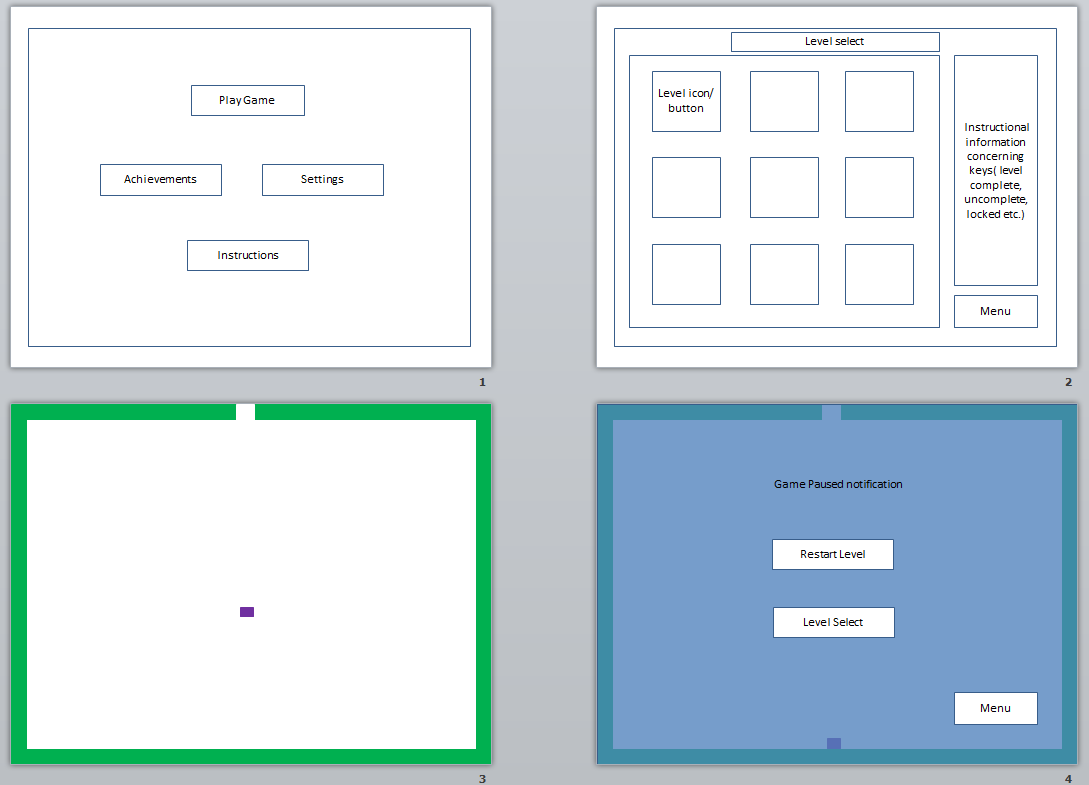
\includegraphics[scale=0.6]{wire1.png}
  \caption{Drawn using Powerpoint, this is the first of a set of wire frames I
used when implementing my game. Each of the menu screens displayed starting
with the main menu and level selection would have the same backgrounds (a cave
image), and each button being blue with a gradient. In the level selection,
levels would be in a three by three grid, all with the number or a padlock image
depending if complete or not. Also having completed a level depending if it was
completed in minimum moves or not would either show a tick if done perfectly a
star shape. The next two wire frames show in play, and also the pause menu when
a user either presses the pause button below the canvas or the 'p' on the users
keyboard.}
   \end{figure}
   \begin{figure}[!ht]
   \centering
   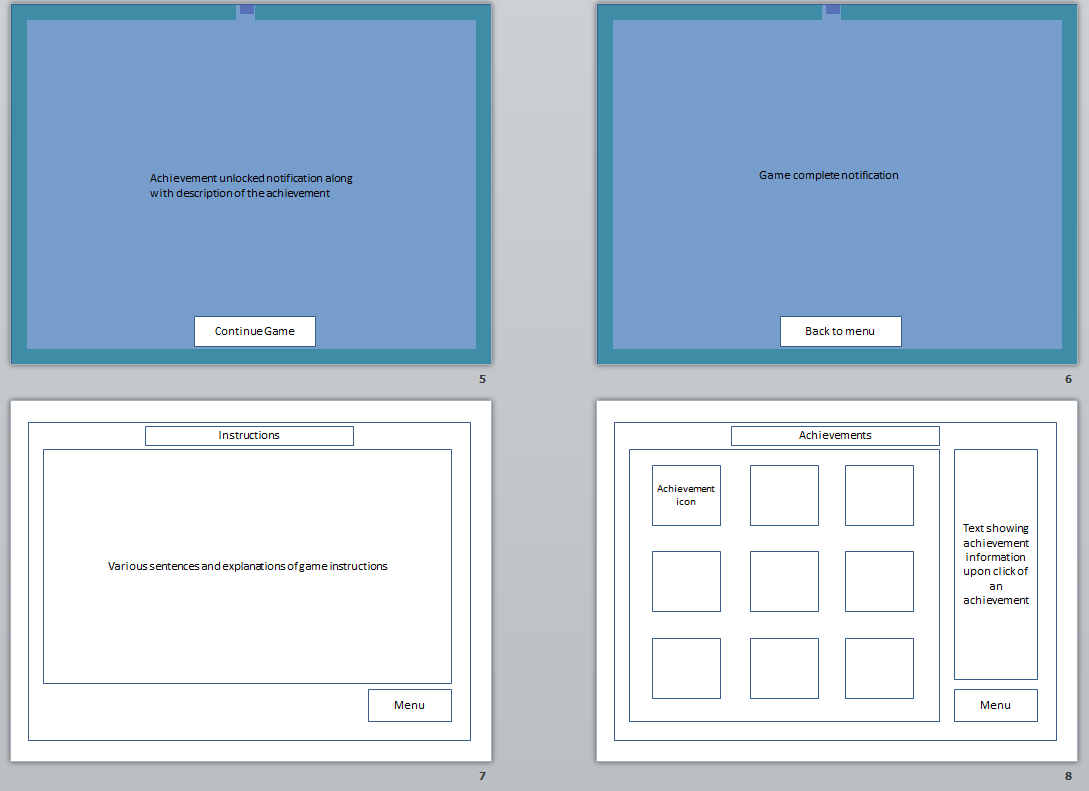
\includegraphics[scale=0.6]{wire2.png}
  \caption{On the next four wire frames, I have shown the user completing an
achievement resulting in a similar semi transparent box that would appear, with
the achievement information followed by a continue game button. On the
instructions page, I have chosen to keep this simple to have the text in a semi
transparent box above the same background as other menus. The text in white, in
bold makes it easier to read. The menu button in the corner would navigate back
to the main menu. As for the achievement frame, this would work similar to the
level selection page.}
   \end{figure}
  \begin{figure}[!ht]
   \centering
   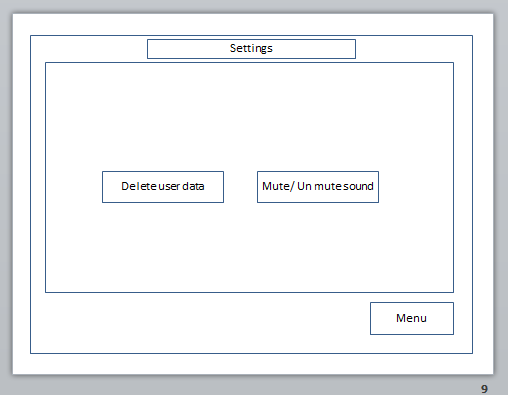
\includegraphics[scale=0.7]{wire3.png}
  \caption{For the final wire frame of this section, the settings page example
shows the options available, being the option to delete achievements and levels
and also the option to mute and un-mute the game. Keeping these as simple as
possible makes the game easier and quicker to use.}
   \end{figure}

\clearpage
\subsection{Use Cases}
I have also chosen to create a set of use case diagrams to provide further
explanations following storyboards. This will show what the options to the
typical user are in-game and within the menus of the game.
\begin{figure}[!ht]
   \centering
   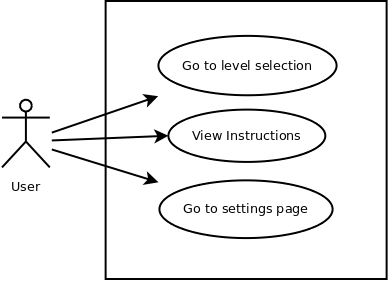
\includegraphics[scale=0.5]{usecase1.png}
  \caption{Use case displaying options to user when game is displayed in
browser}
   \end{figure}
   \begin{figure}[!ht]
   \centering
   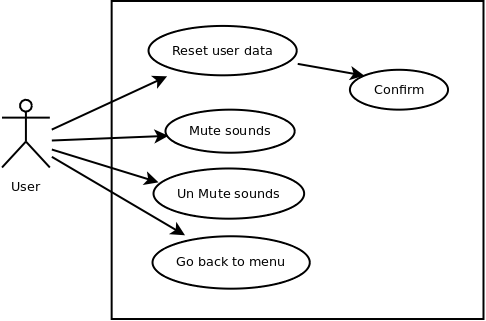
\includegraphics[scale=0.5]{usecase2.png}
  \caption{Within the settings of the menu, the user can choose these options,
and when resetting user data can choose to confirm or not. This avoids
accidental loss of data.}
   \end{figure}
   \begin{figure}[!ht]
   \centering
   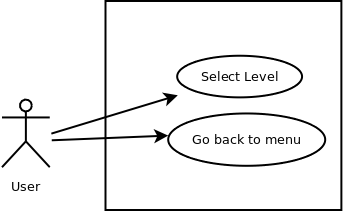
\includegraphics[scale=0.5]{usecase3.png}
  \caption{When in the level selection menu, the user can choose to play a level
or go back to the menu.}
   \end{figure}
   \begin{figure}[!ht]
   \centering
   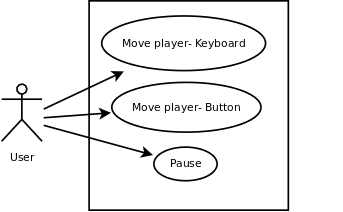
\includegraphics[scale=0.9]{usecase4.png}
  \caption{There is two methods of moving a player, and also the option to pause
the level in-game.}
   \end{figure}
   \begin{figure}[!ht]
   \centering
   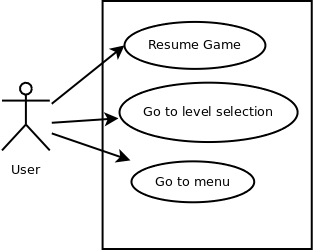
\includegraphics[scale=0.6]{usecase5.png}
  \caption{This simply shows options within the pause menu. The user can resume,
choose another level, or go back to the main menu.}
   \end{figure}
\clearpage
\begin{landscape}
  \subsection{Story Boards}
\begin{figure}[!ht]
   \centering
   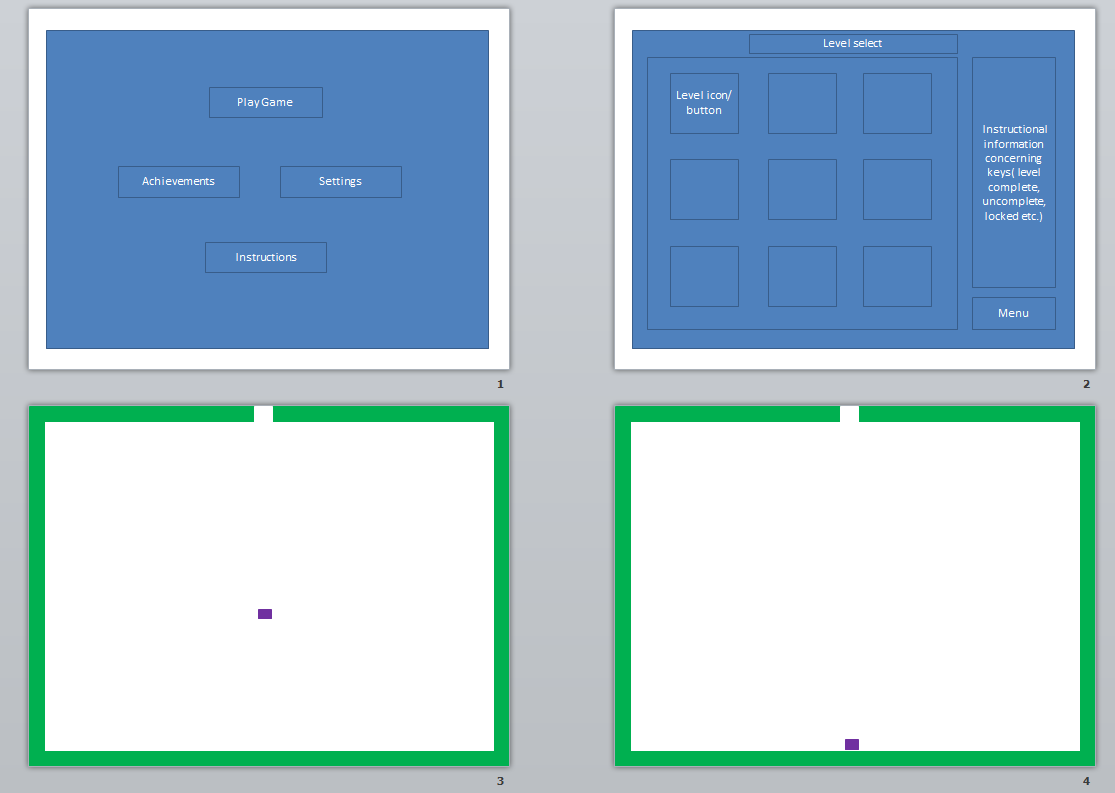
\includegraphics[scale=0.65]{story1.png}
  \caption{The story board displayed below shows the first four stages of
playing a level within the game. As you can see, the user would firstly select
the 'play game' then choose an available level on the selection menu. Once this
is done, the user then moves the player around the maze. In state 4, the user
has hit a wall resulting in the stopping of movement of the player. The next
move is awaited.}
   \end{figure}
\end{landscape}
\clearpage
\begin{landscape}
\begin{figure}[!ht]
   \centering
   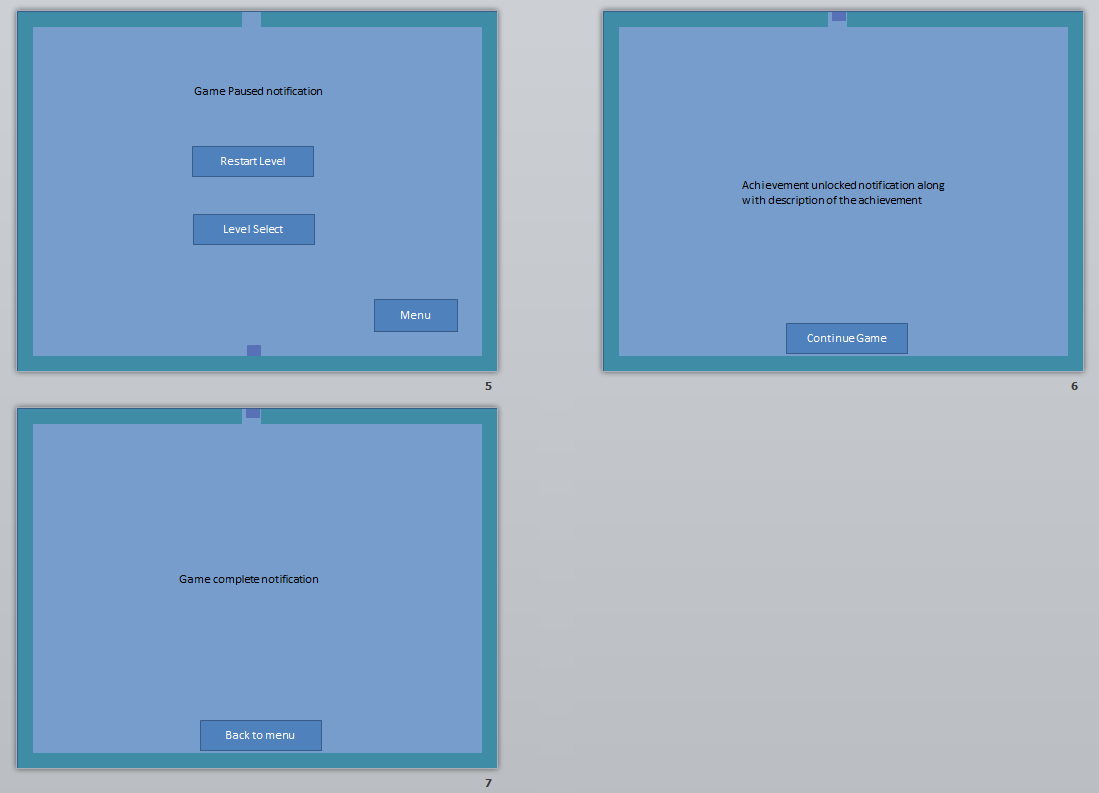
\includegraphics[scale=0.8]{story2.png}
  \caption{In the next three stages of the storyboard intended to show the way a
user would navigate through playing the game, I have firstly shown the paused
menu, followed by a user completing a level triggering an achievement. After
clicking continue, the user would then move to the next level. In the final
storyboard, the game is complete and the user would press the menu button to
return top the menu.}
   \end{figure}
\end{landscape}
\clearpage
\subsection{Javascript Class Diagram}
\begin{figure}[!ht]
   \centering
   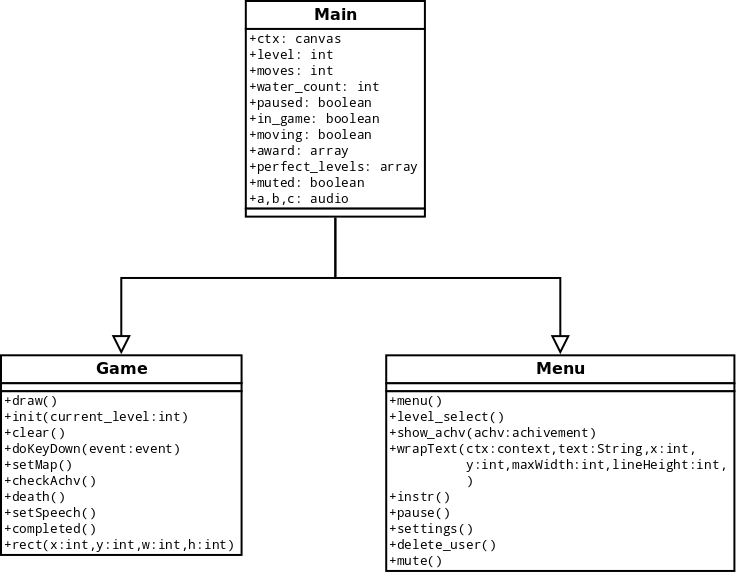
\includegraphics[scale=0.5]{class.png}
  \caption{Tee first class, which is simple set up code within the game page
creates all the variables used in the functions within the game. These are all
public to make them easily accessible. Key variables here hold the level number
currently playing, the boolean to check if the user has paused the game or not,
and if the sound is muted. The other classes linked from this create the menus
and game itself. Within the game, the draw method draws the map after every few
milliseconds as the position of the player moves, and the clear function
refreshes the canvas before every draw. Other methods here check the
achievements, pauses, deaths etc.}
   \end{figure}
  \clearpage

\subsection{Javascript State Diagrams}
The final set of diagrams in this section are my state diagrams. These help show
the way a user runs through a set of methods to get to a certain feature in my
game. For instance, choosing to play, selecting a level and then playing it are
all steps towards beginning a level.
\begin{figure}[!ht]
   \centering
   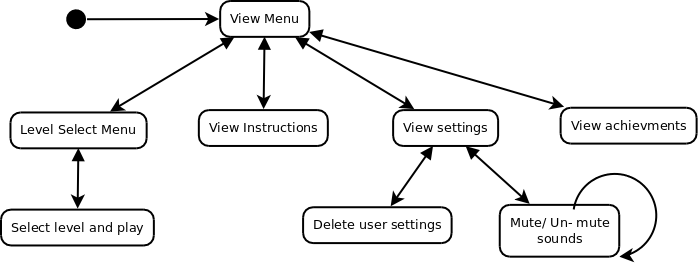
\includegraphics[scale=0.5]{state1.png}
  \caption{THis simply shows the transitions between different states the user
can get the system into. In the menu for instance, the user can go to a range of
menus and get easily back to the main menu at any time. }
   \end{figure}
   \begin{figure}[!ht]
   \centering
   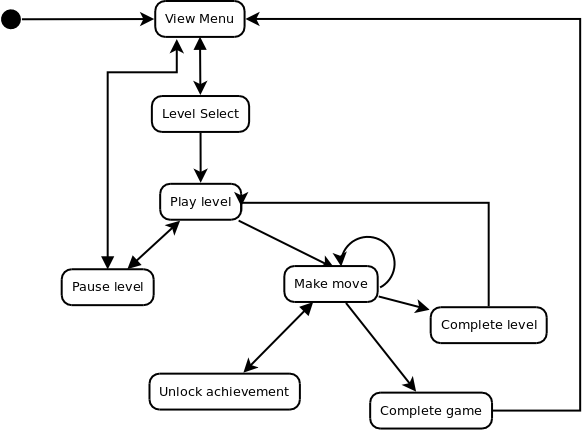
\includegraphics[scale=0.5]{state2.png}
  \caption{The last diagram here shows the run through of playing a level. When
inside a level after making a move, the user can either make another move,
unlock an achievement, complete the game or complete a level. In the instance of
completing a level,the user would be taken back to the main menu.}
   \end{figure}
    \clearpage

\section{Technical Overview}
Making the game in Javascript meant that being a client side language, the game
would initiate and run completely depending on the users computer. A clear
advantage I found was that the speed in which the game would load would be
considerably faster. This is because any elements of the game that would usually
be needed would have to be sent from the server and this would take more time
opposed to  having the script already loaded ready for running. \\
\\Another set of reasons I preferred Javascript for the implementation of my
game over alternatives possible such as Java or Flash would be compatibility.
Because these are more advanced styles of game programming, they are also more
dependent on better, up to date browsers that  must be equipped with the correct
software to run the scripts. This could cause a problem for a user if they did
not have flash/ Java installed, whilst my game being Javascript avoids this
because all browsers already are ready to run these type of scripts. Linking
this with the choice for using client side over server side, I can also say that
the choice to store data such as achievements on the client side using local
storage will always ensure that a users data is not lost, unlike if a server
went down and their data was not their own responsibility.\\
\\As a short note about external Javascript libraries, I chose not to implement
any of these. This was due to me then being able to create functions area
specific for what I needed, and ones which I could change easily.

\section{Software Testing}
Below, I have created a set of sub sections that look at the different browsers
I tested my site and game on, speed tests of my site, to ensure my code and game
runs to the best possible efficiency.

\subsection{Browser Compatibility}
The first aim after I had implemented my game and website was to ensure that it
ran correctly on a range of different browsers. To begin, I already knew that
because the game was placed within an HTML5 element, it would not function on
Internet Explorer. Because I could not avoid this, I chose to simply place a
piece of text where the canvas would be informing the user of this issue.\\On
the following pages are the resulting screenshots of running my game in a range
of different browsers:
   \begin{figure}[!ht]
   \centering
   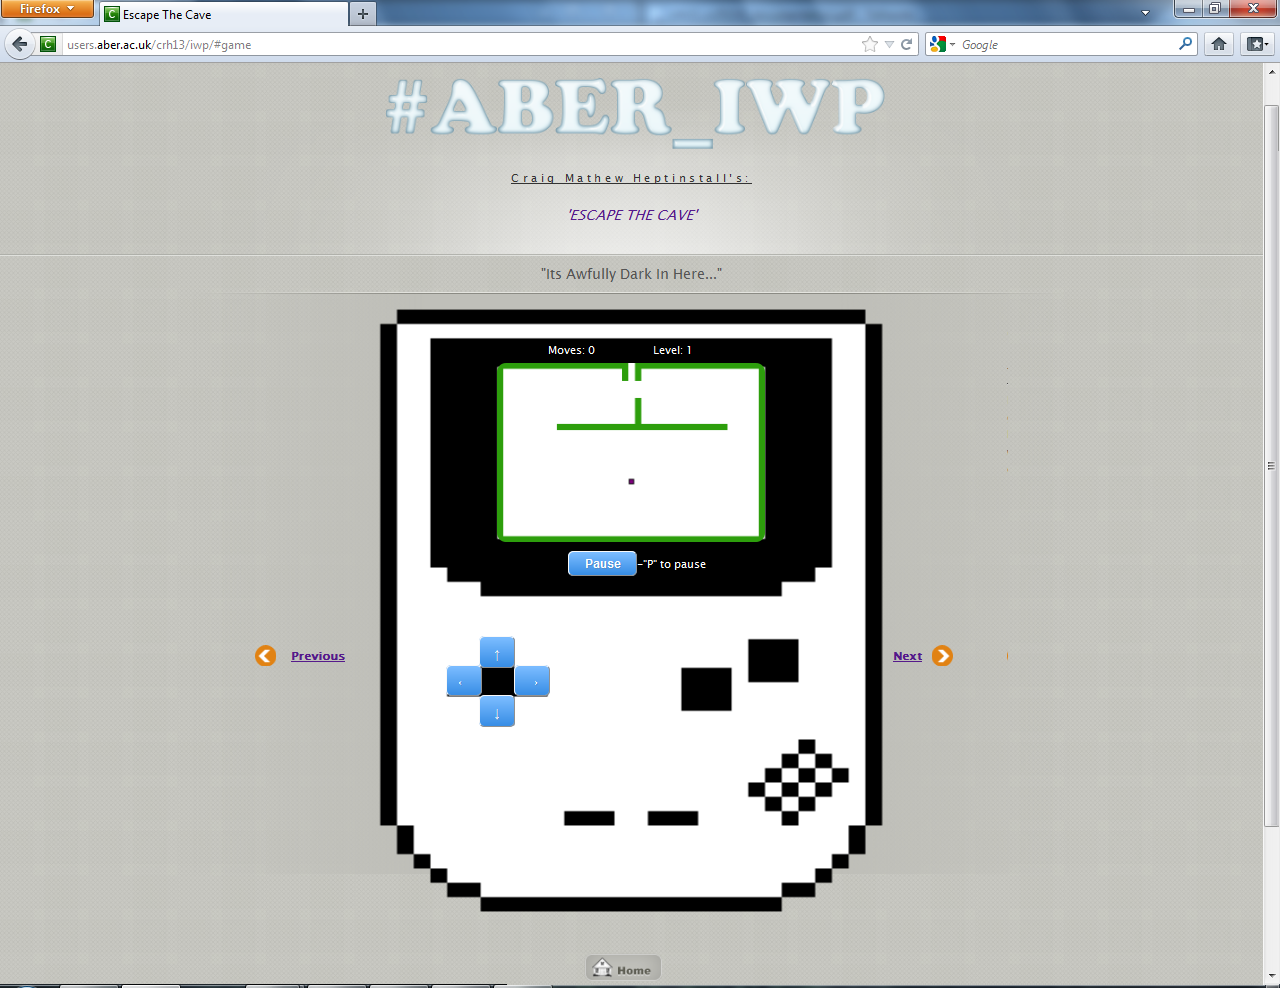
\includegraphics[scale=0.35]{firefox.png}
  \caption{(\emph{Firefox})- This browser displayed the game and site features
very well, including the gradients on the buttons. When playing the game in
this browser, I did find Firefox was slightly slower than the other browsers at
handling Javascript, but the game was perfectly playable.}
   \end{figure}
\clearpage
 \begin{figure}[!ht]
   \centering
   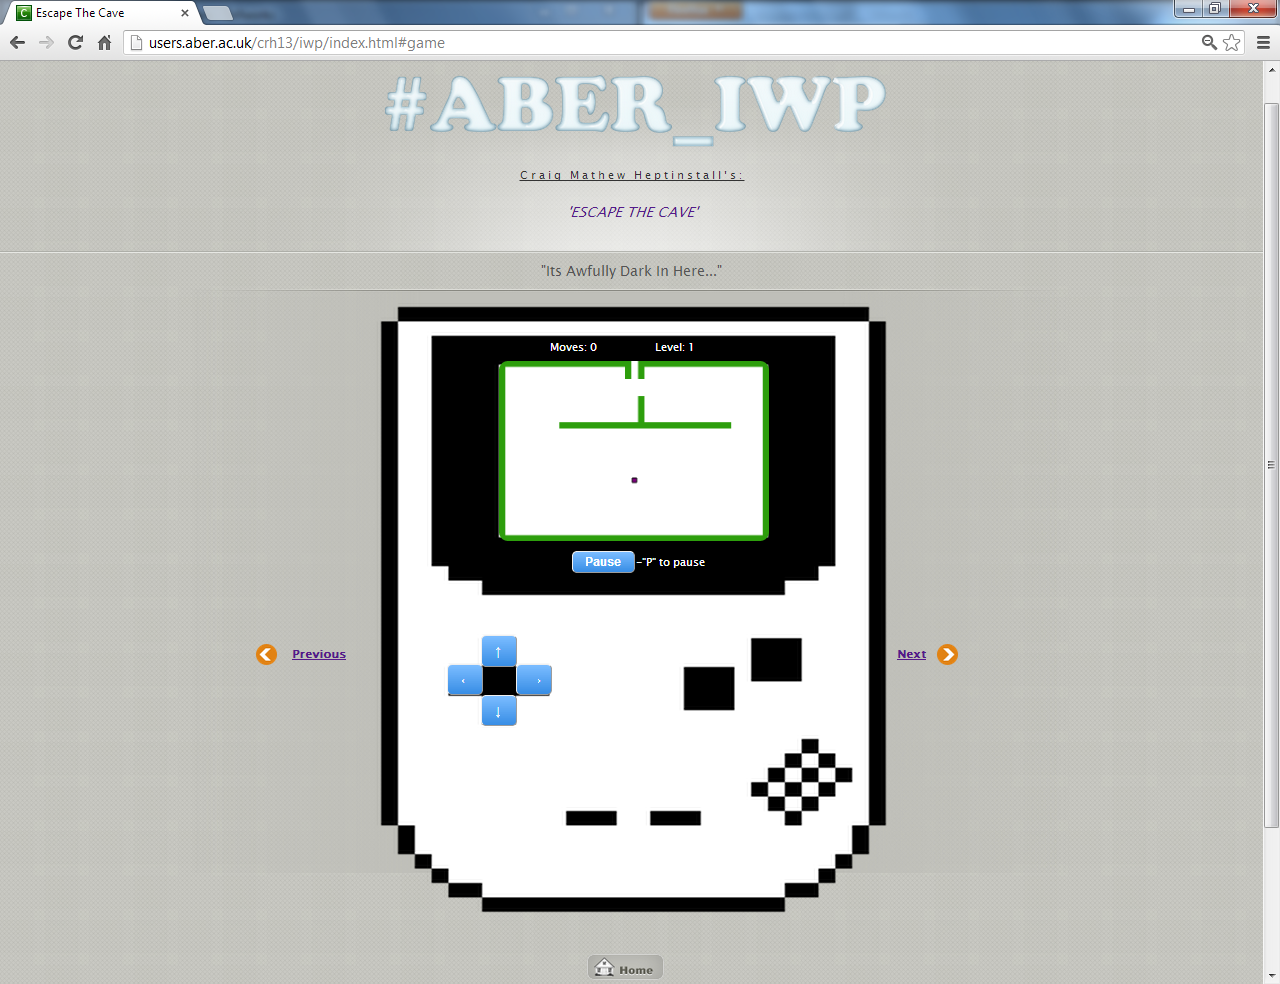
\includegraphics[scale=0.4]{chrome.png}
  \caption{(\emph{Chrome})- The Google Chrome browser handled the game very
well, at a much higher speed than that of Firefox and SeaMonkey and again also
allowed for the gradient style on each of the buttons. I found Chrome loaded
in-play images faster too, so when advancing to a new level it loaded faster
than most others.}
   \end{figure}
   \begin{figure}[!ht]
   \centering
   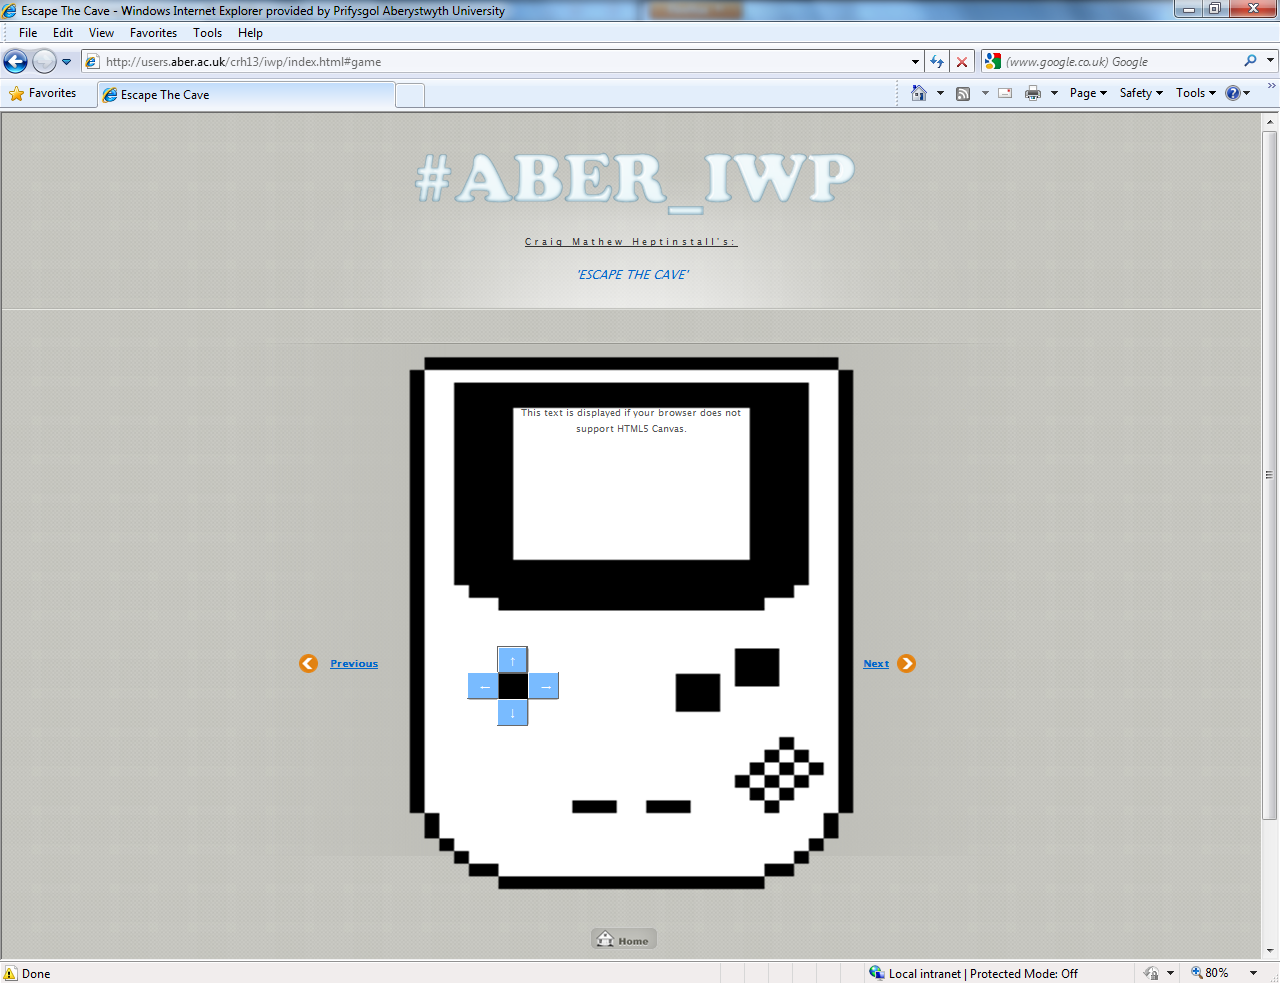
\includegraphics[scale=0.4]{ie.png}
  \caption{(\emph{Internet Explorer})- The only browser not to display the game,
Internet explorer failed to run the canvas which in turn produced the text
telling the user it could not run on that platform. In addition to this, IE also
did not allow for the gradient on buttons, instead being plain rollover
buttons.}
   \end{figure}
\clearpage
 \begin{figure}[!ht]
   \centering
   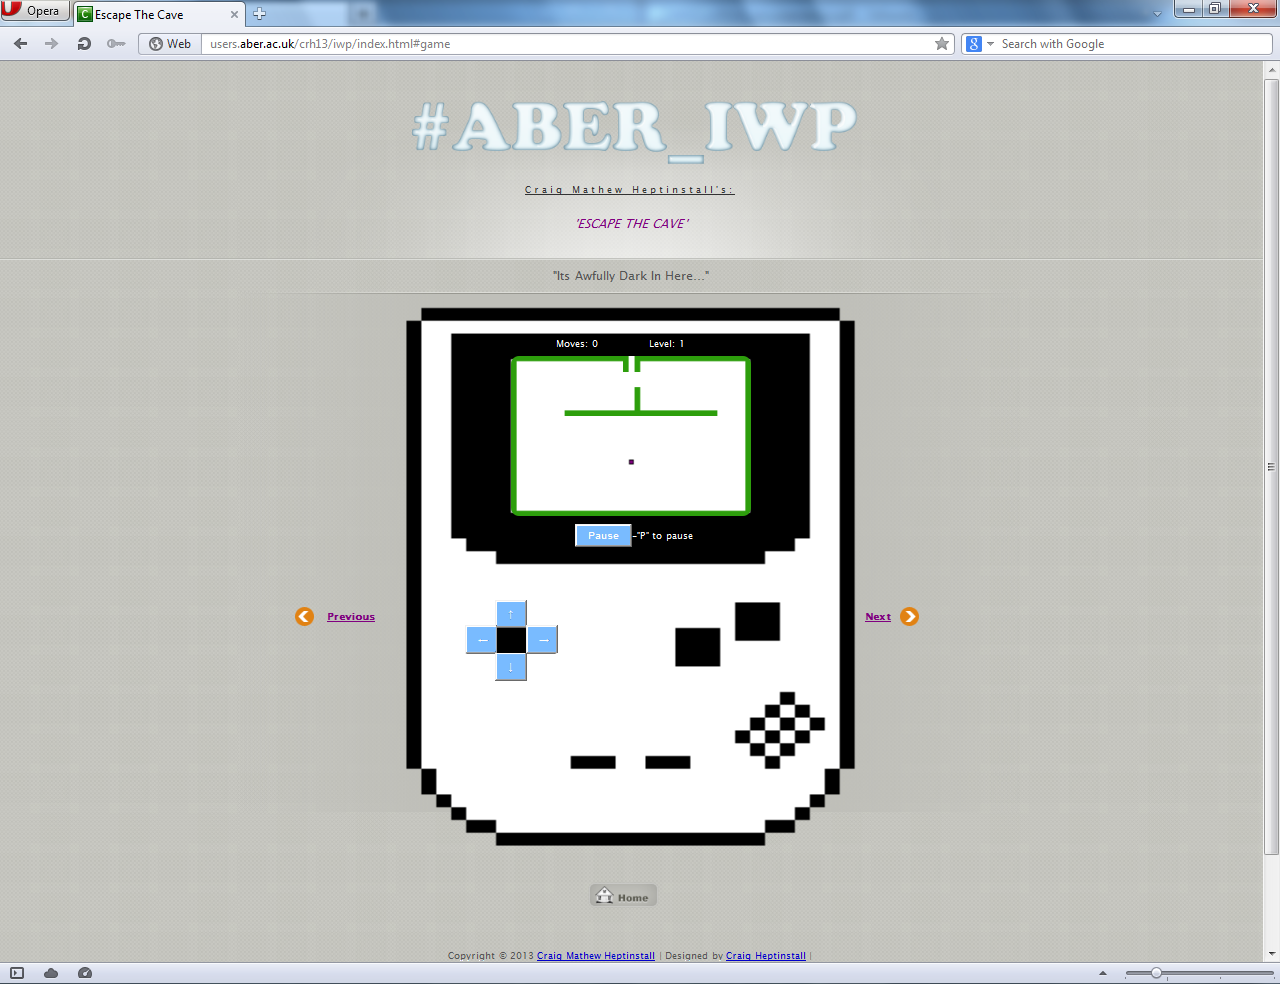
\includegraphics[scale=0.38]{opera.png}
  \caption{(\emph{Opera})- The second fastest in terms of playability speed
concerning the Javascript abilities, Opera loaded images very fast compared to
other browsers. Again, button gradients did not appear on opera and showed up as
just plain rollover buttons. Although all browsers loaded the music roughly the
same speed (except IE), opera seemed slightly quicker.}
   \end{figure}
   \begin{figure}[!ht]
   \centering
   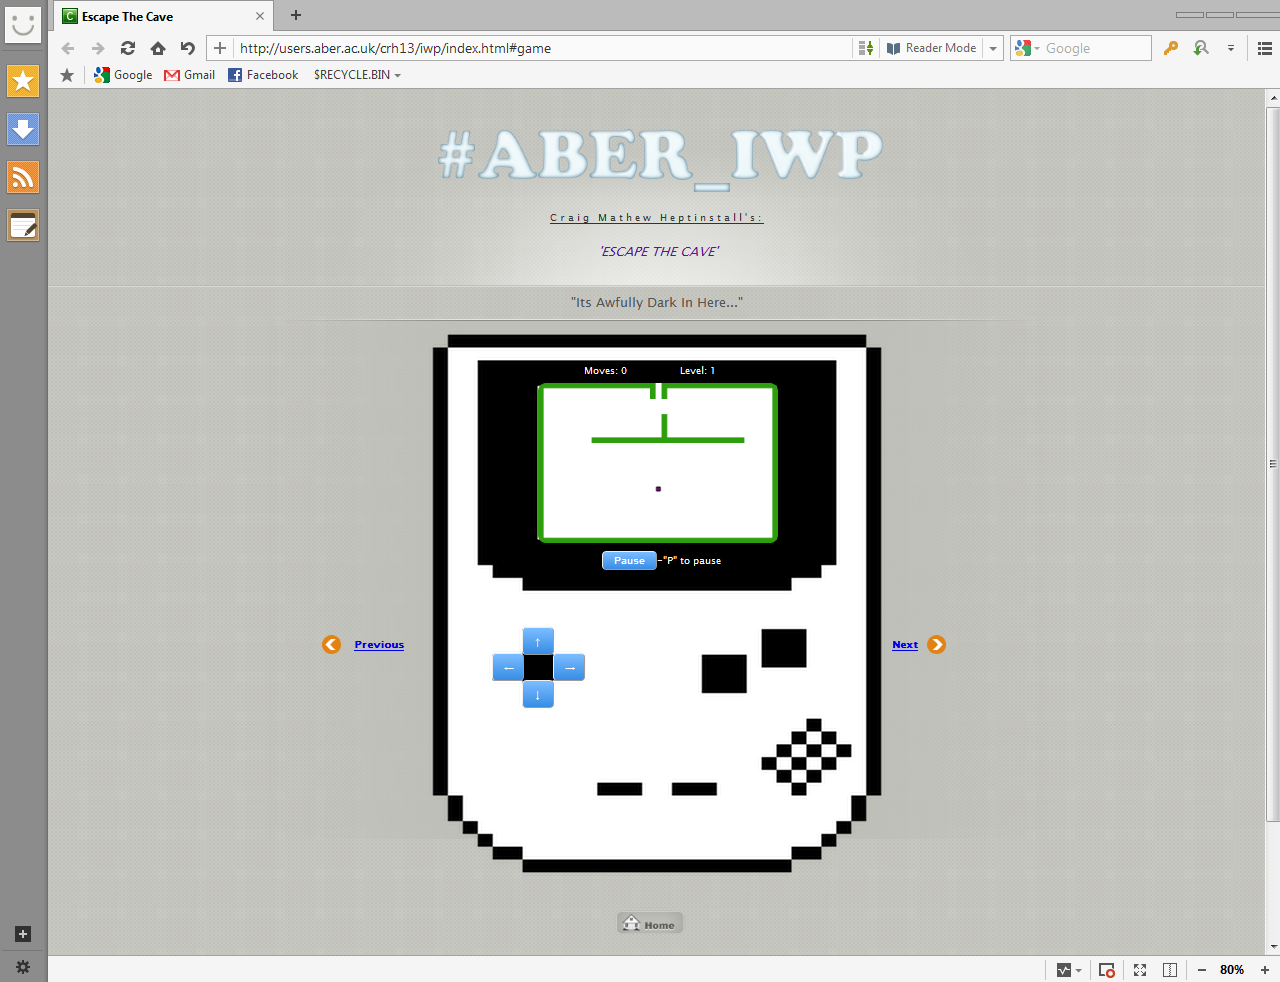
\includegraphics[scale=0.4]{maxthon.png}
  \caption{(\emph{Maxthon})- From testing each browser on different computers, I
have found that this browser was the fastest in terms of running the Javascript,
resulting in smoother and faster game play. Maxthon also allowed for gradients
upon any buttons in the menus or on the site.6}
   \end{figure}
 \begin{figure}[!ht]
   \centering
   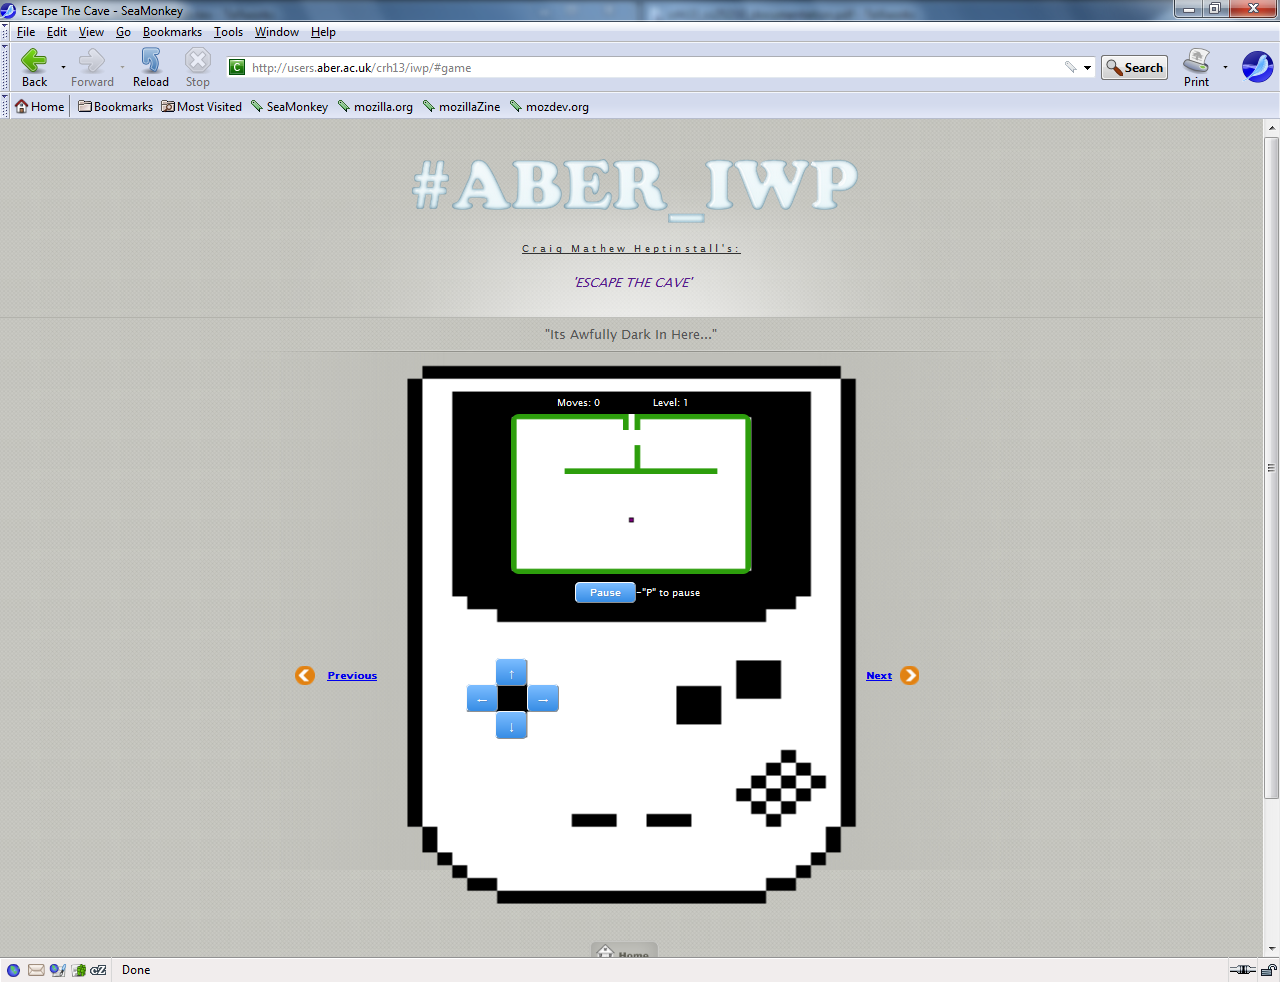
\includegraphics[scale=0.4]{seamonkey.png}
  \caption{(\emph{SeaMonkey})- The slowest of the browsers that played the game,
SeaMonkey did allow for gradients, but ran slightly slower at times, for
instance the player square object would not run across the screen in a
completely smooth manner.  }
   \end{figure}
\clearpage
Following on from desktop browser testing, I also implemented a mobile test of
the game. A good mobile testing site was used here \cite{mobile}. I have shown
this below:\\
 \begin{figure}[!ht]
   \centering
   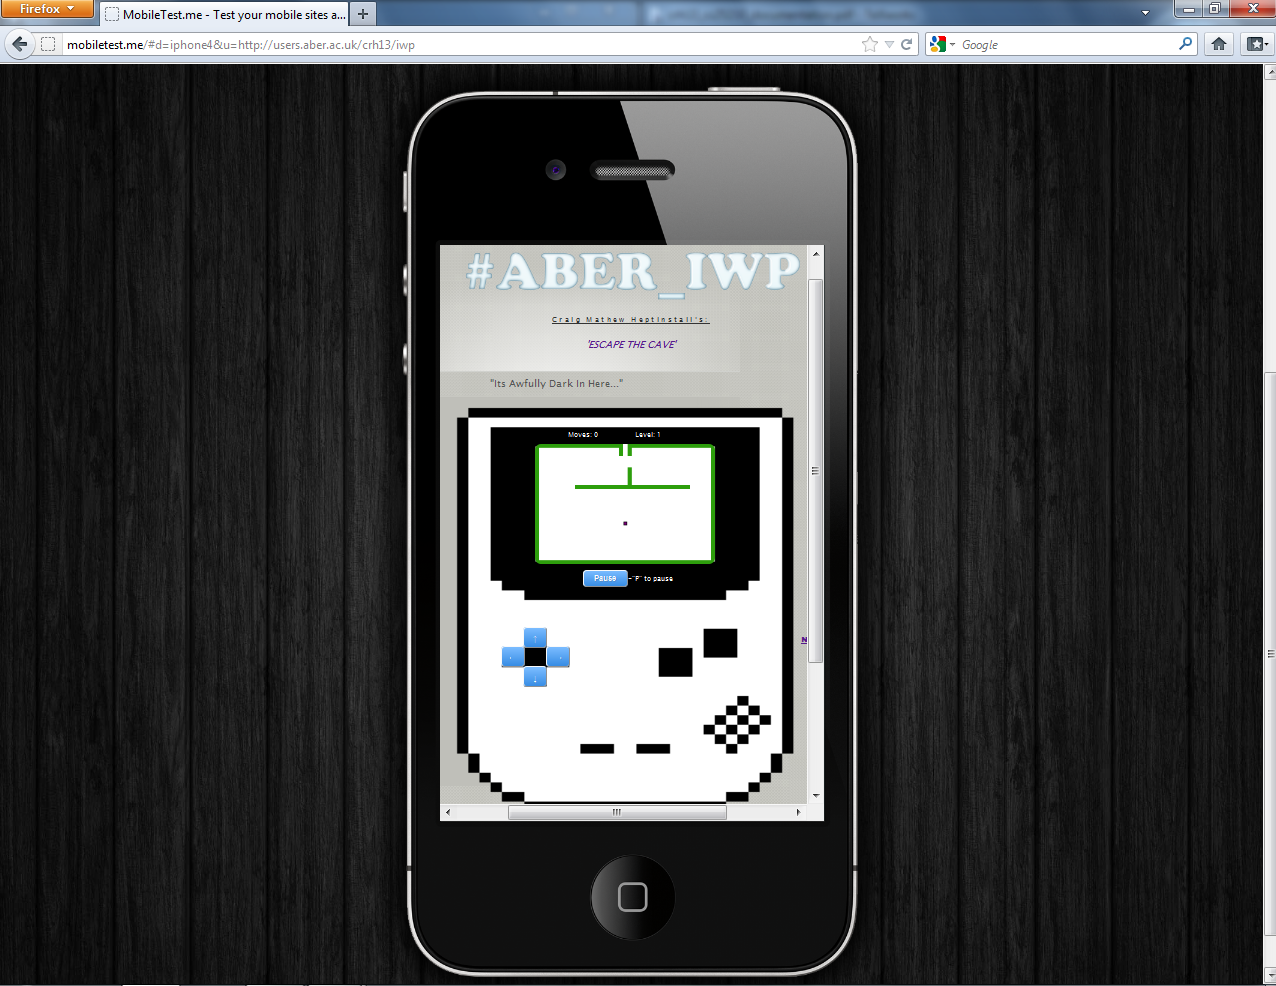
\includegraphics[scale=0.4]{iphone.png}
  \caption{As you will also see if that on my own phone type, the game ran fine
and allowed me to play the game properly using the directional buttons placed on
the page. I wanted to get a wider scope of tests here, so I also did some tests
on a number of other phones to see how the site performed.}
   \end{figure}
 \begin{figure}[!ht]
   \centering
   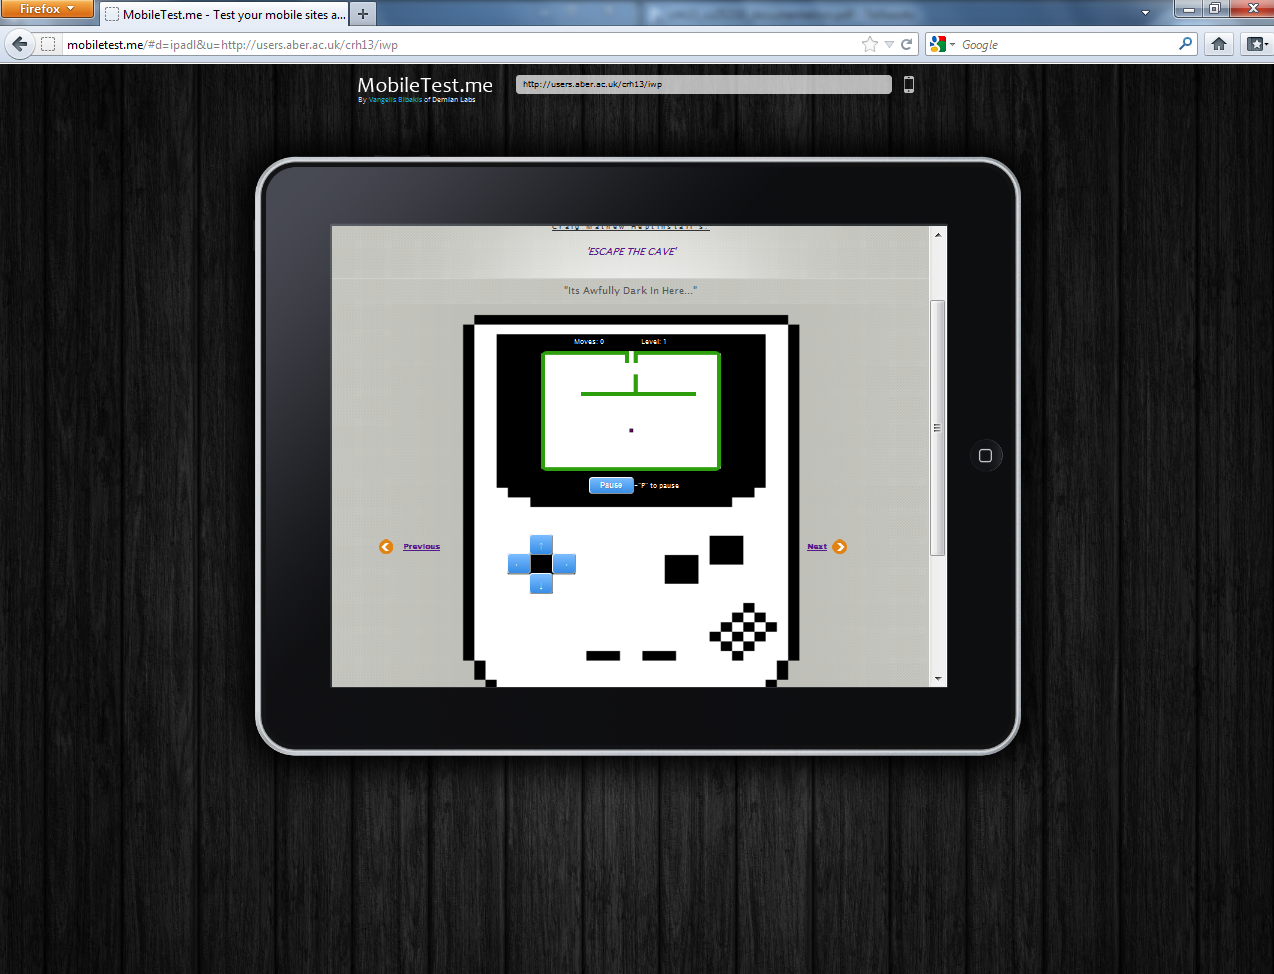
\includegraphics[scale=0.35]{ipad.png}
  \caption{The iPad, running the same software as that of the iPhone, shows that
the game again ran just as well. this time because of the size of the screen
allowed the game to be made bigger. In both cases, the sound played fine
including the use of the mute and un-mute functions.}
   \end{figure}
 \begin{figure}[!ht]
   \centering
   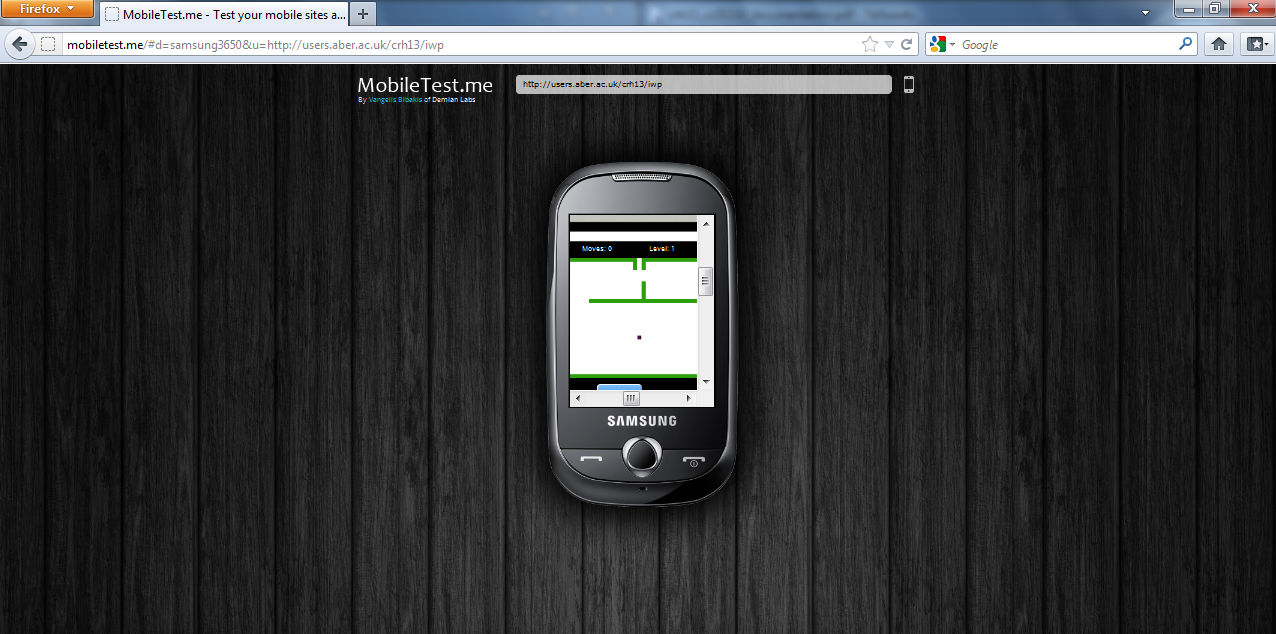
\includegraphics[scale=0.5]{sony.png}
  \caption{I wanted to try the game on a different phone and browser all
together here, this time being a Samsung. I used an older phone here to see the
capabilities of the browser and if it could support the canvas element. As you
can see, the game again runs fine, although the only issue here was the screen
was slightly too small to fit the whole canvas in and makes the game very hard
to play. The sound did not load on this phone unlike the previous two.}
   \end{figure}
\\I would like to note here that when running my game offline on a desktop, that
in Chrome the game did function. This was caused by a work around I had to use
for this browser concerning 'CrossOrigin'. I had to use this code to ensure
Chrome did allow multiple image locations for the same image object. \\
\\
 

\begin{figure}[!ht]
\centering
\begin{tabular}{|c | c | c | p{8cm}|}

\hline

OS & Browser & Works? & Description \\

\hline
Windows & Chrome & Yes & Worked smoothly, all sounds loaded and also loaded
button gradients. Note: Did not work offline due to Cross Origin problem.\\
Ubuntu & Chrome & Yes & Same results as on Windows.\\
Windows & Firefox & Yes & Worked well, although not as fast as Chrome's ability
to run the Javascript code.\\
Ubuntu & Firefox & Yes & Exact results as the Windows version.\\
Windows & Opera & Yes & Worked fine, although gradients on buttons did not show,
instead showing plain buttons.\\
Ubuntu & Opera & Yes & Exact same results as the Windows version.\\
Windows & IE & Yes & The game did not load at all because of the canvas element
not being implemented. Showed text telling user of tis instead.\\
Windows & Safari & Yes & After a small bug I found when first testing this
concerning the image of the map not loading after resetting the level, I fixed
this by creating a new Map image object every time the image loads. Works
completely fine now.\\
Mac & Safari & Yes & Same results as on Windows.\\
\hline


\end{tabular}
\caption{This table shows general results of some of the tests from my desktop
browser tests, but under different operating systems. For instance, although I
showed all the major browsers, this was only under Windows. To get a better
scope, I have tested some browsers in both Windows, Ubuntu and also Mac Os.
Testing in different operating systems is important because for instance, the
libraries concerning types of fonts are not available in Ubuntu as widely as
they are in Windows.}

\end{figure}
\clearpage

\subsection{Website Testing}
One of many possible testing methods was to use the jslint website \cite{jslint}
tool that allowed me to easily paste in my code, then find out any errors or
warnings that could affect my site. A frequent set of warnings that appeared was
where I had seemed to miss out the ';' symbol at end of lines of code.
validation of site and js checker site
\subsection{Alternative Testing}
Looking at any other alternative tests, a tool such as JSUnit (Javascript Unit
Tests) \cite{jsunit}, would allow me to perform code tests alike JUnit would for
Java.
   \begin{figure}[!ht]
   \centering
   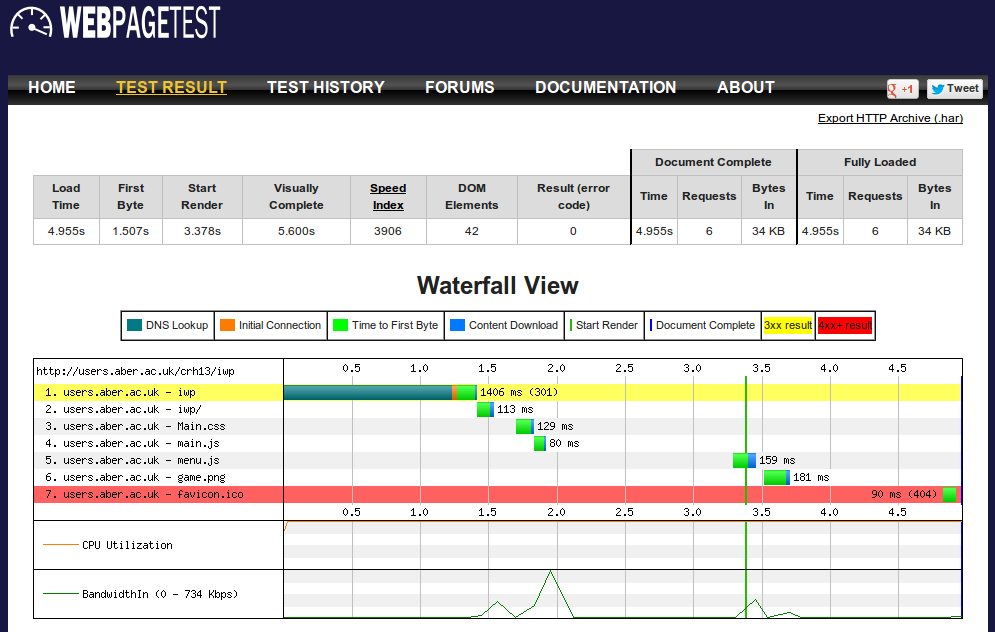
\includegraphics[scale=0.5]{speed.png}
  \caption{Diagram gained from webpage test site \cite{webpagetest} showing
waterfall loading times for the page. As you can see, the page loads including
all Javascript and images in around 4 seconds. This is average for a page before
a user leaves so I have showed here my page loads with good speed.}
   \end{figure}

\section{Reflections and Future Work}
If I had of used methods such as flash, Java FX or Silverlight, I believe that I
could have created a higher quality game with more special effects such as 3D
like maps. Because Javascript is dependent on the users machine, more checking
can seriously slow the game down.\\
\\If I had have used some server side languages such as PHP on my site it would
have allowed for highscores, but because of the nature of my game, I am still
unsure how I would use highscores to my advantage. With the use of local storage
from HTML5, I still think client side sufficed here to meet the needs of my
game.\\
\\If I had more time, or continued to work on this game, it would be very easy
to implement new levels and achievements, and add a sliding menu to my game,
giving it the sliding menu and level amounts similar to well known games like
'Angry Birds'.  Monetizing the game could be done with special upgrades, such as
hints and tips, where users could earn or buy these tips to help them through
levels. Implementing this as a mobile application this would also provide a
means of creating money, and increase availability for a wider range of users.\\
\\As a final point, an improvement I would have liked to make if more time was
available would be to look at creating maps on the fly rather than by images.
This could be done using many vectors to draw the maps which in turn would
increase loading times of levels dramatically. 

\vspace{10mm} 
\begin{center}
\framebox[1.4\width]{Word Count (Excluding figure captions): 1081 \cite{count}}
\end{center}

\section{REFERENCES}

\begin{thebibliography}{9}

\bibitem{webpagetest} http://www.webpagetest.org. Webpage loading test program.
AOL. 2008
\bibitem{jslint} http://www.jslint.com. Javascript Checker. V1.5.2. Doxygen.
2007
\bibitem{jsunit} http://jsunit.berlios.de/. Javascript test suite for testing
methods. Douglas Crockford. 2002
\bibitem{mobile} http://mobiletest.me/. Online Interactive Mobile tests site.
Vangelis Bibakis of Demian Labs.
\bibitem{count} http://app.uio.no/ifi/texcount/online.php. Online tex word
count. Einar Andreas Rodland. 2012.
\end{thebibliography}

\section{DOCUMENT HISTORY}

\begin{tabular}{|l | l | l | l | l |}

\hline

Version & Date & Changes made to Document & Changed by \\

\hline
1.0  & March 25, 2013 & Creation of first draft of document & Crh13\\
1.1  & April 15, 2013 & Addition of diagrams & Crh13\\
1.2  & April 22, 2013 & Spell checking of document & Crh13\\
1.3  & \today & Release version & Crh13\\
\hline


\end{tabular}
\end{document}

\clearpage

\end{document}